%
% NOS
%
% Aleph Objects Firewall
%
% Copyright (C) 2014, 2015, 2016 Aleph Objects, Inc.
%
% This document is licensed under the Creative Commons Attribution 4.0
% International Public License (CC BY-SA 4.0) by Aleph Objects, Inc.
%
There are a lot of operating systems to consider...


\section{Debian}
 \href{https://www.debian.org/}{Debian}

We use Debian for nearly everything else. It could easily be used as a router/firewall. There are better, more tuned options.


\section{OpenBSD}
 \href{https://www.openbsd.org/}{OpenBSD}

We are using OpenBSD right now for our firewall. It is very reliable and secure. Few people know how to administer it. It is all command line editing of
firewall configuration files. We are potentially switching away from it to get something easier to use and that has more analytics.


\section{Gentoo}
 \href{https://www.gentoo.org/}{Gentoo}

Can be tuned in.


\section{FreeBSD}
 \href{https://www.freebsd.org/}{FreeBSD}

Solid OS. Can use OpenBSD's pf, iirc. Same problem as with OpenBSD, few admins know it.


\section{NetBSD}
 \href{https://www.netbsd.org/}{NetBSD}

Solid OS. Can use OpenBSD's pf, iirc. Same problem as with OpenBSD, few admins know it.


\section{Alpine Linux}
 \href{https://www.alpinelinux.org/}{Alpine} --- ``Small. Simple. Secure. Alpine Linux is a security-oriented, lightweight Linux distribution based on musl libc and busybox.''

Download and install .iso to USB. Boot from USB, do text install onto HD. The installer looked very much like OpenBSD and was quite terse, but worked fine.
The installed system is a basic lean GNU/Linux installation. Firewall configuration is text based. Looks nice, but not many features, except lightweight.
Similar to OpenWRT in that way, except no web GUI, AFAICT.


\section{clearOS}

\begin{figure}[h!]
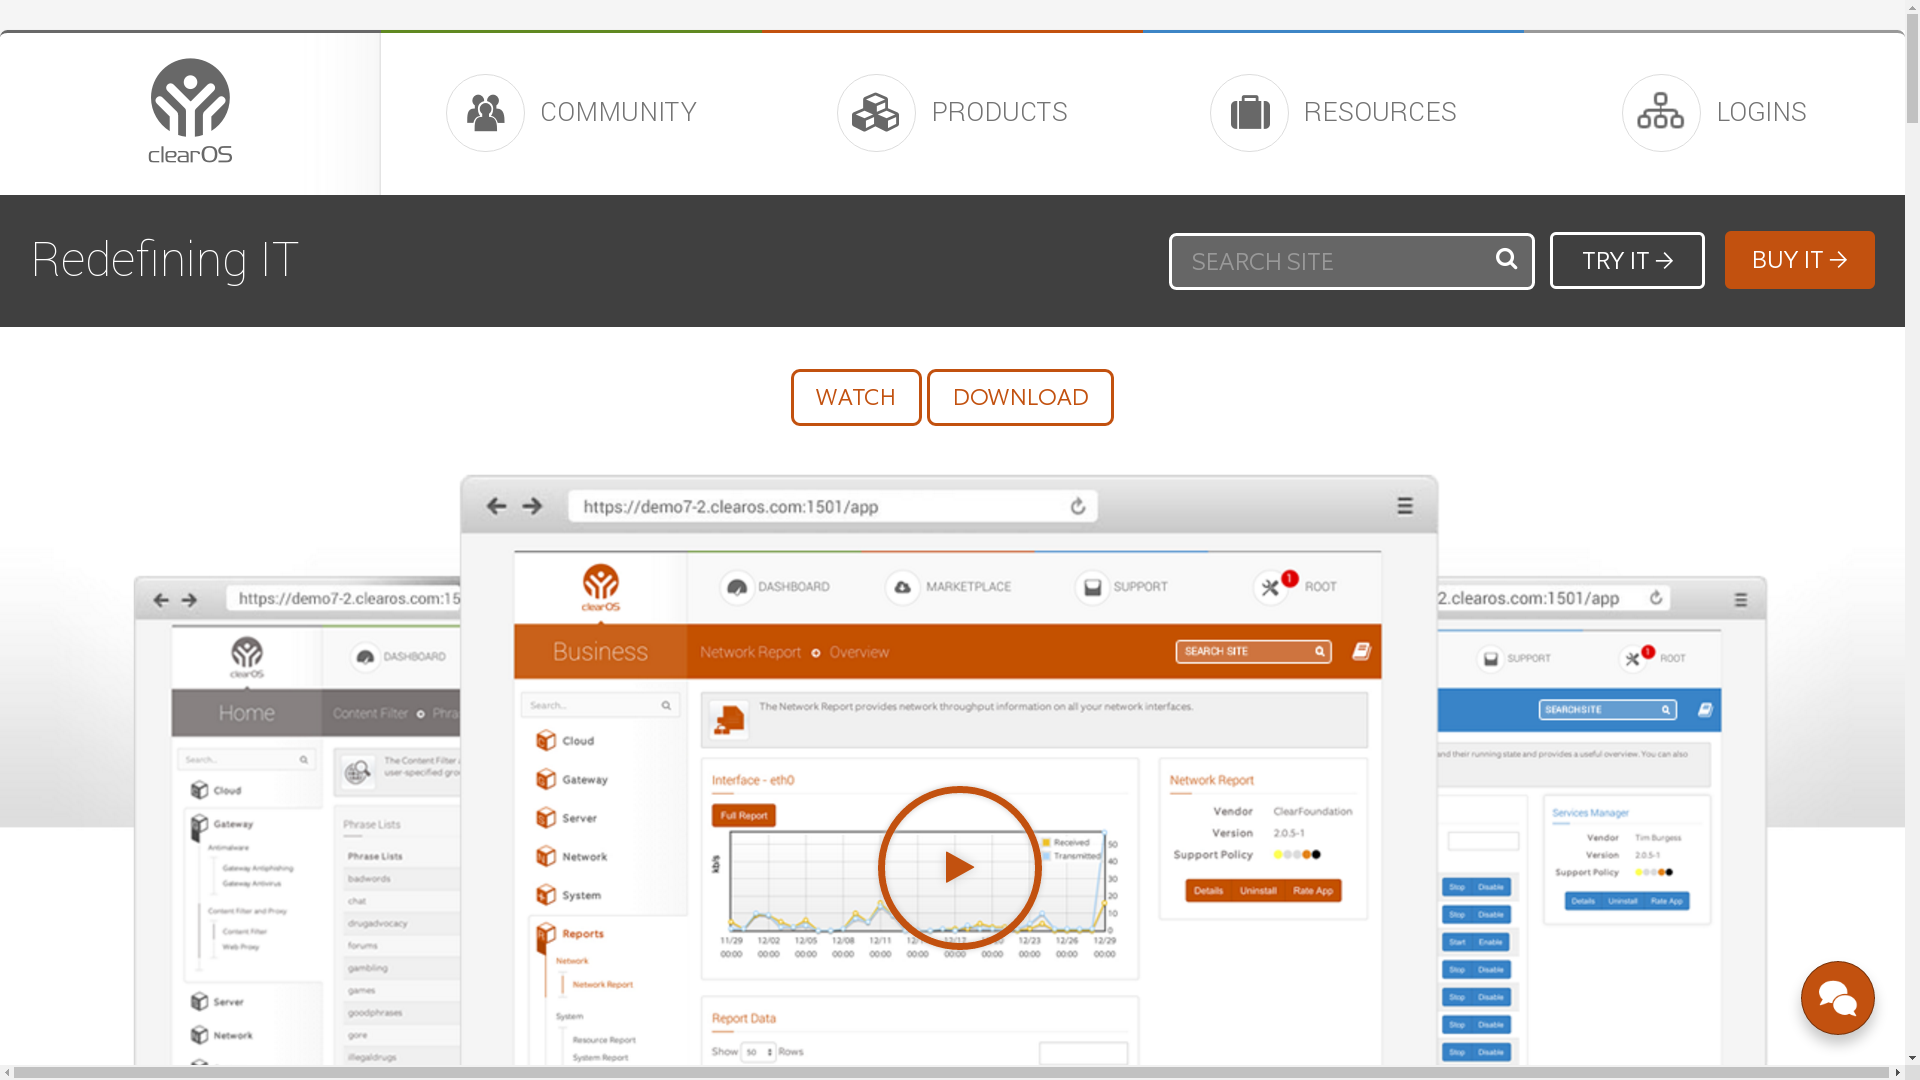
\includegraphics[keepaspectratio=true,height=1.10\textheight,width=1.00\textwidth,angle=0]{www-clearos.png}
 \caption{clearOS Website}
 \label{fig:www-clearos}
\end{figure}

\href{https://www.clearos.com/}{clearOS} --- ``ClearOS is an operating system for your Server, Network, and Gateway systems. It is designed for homes, small to medium businesses, and distributed environments. ClearOS is commonly known as the Next Generation Small Business Server, while including indispensable Gateway and Networking functionality. It delivers a powerful IT solution with an elegant user interface that is completely web-based.''

\begin{itemize}
 \item Overall, very very nice, very clean with many features.
 \item Baitware is the only thing holding this back.
 \item The web interface never crashed or caused issues.
 \item Usage is stable.
 \item Latest release: 7.2.0
 \item Release Date: March 7, 2015.
 \item Package Updater: yum
 \item Base OS: Fedora? CentOS?
 \item Easy GUI install
 \item Has enterprise (baitware?) version.
 \item Has enterprise hardware.
 \item Web based configuration system started on first boot
 \item Web wizard has option to select Community or non-free versions.
 \item Web wizard has system registration for a marketplace for apps. Have to register?
 \item Registering set ``Software End-of-Life" to August 31, 2018.
 \item Lots of phone-home activity with marketplace and registration....
 \item Simple ``Update All" button to update system (with yum, afaict).
 \item Very clean, overall.
 \item Wide variety of ``Apps" in the Marketplace that are GPL.
 \item Non-free plugins are listed along free ones. The owncloud plugin is non-free.
 \item Most apps don't have any ratings,
 \item The default ``Exception Sites" whitelist had their clear*.com sites and a few *.microsoft.com.
 \item Has optionally transparent web proxy.
 \item Installed many Apps, and it was all very clean.
 \item clearOS gets pwned, we get pwnd? Yes.
 \item Need to create account to get to knowledge base ?
 \item Actual firewalling rules (e.g. block just these devices from everything but port 443) aren't so strong.
 \item There doesn't appear to be a way to say ``just allow port 22 from NNN"...
 \item A lot of great setup.
 \item MultiWAN --- Nice, but simple load balancing between multiple upstreams.
 \item No fail over to another router (ala CARP).
 \item dhclient (?) overwrites DNS addresses, no place to set static (?!?)
\end{itemize}


\section{IPCop}
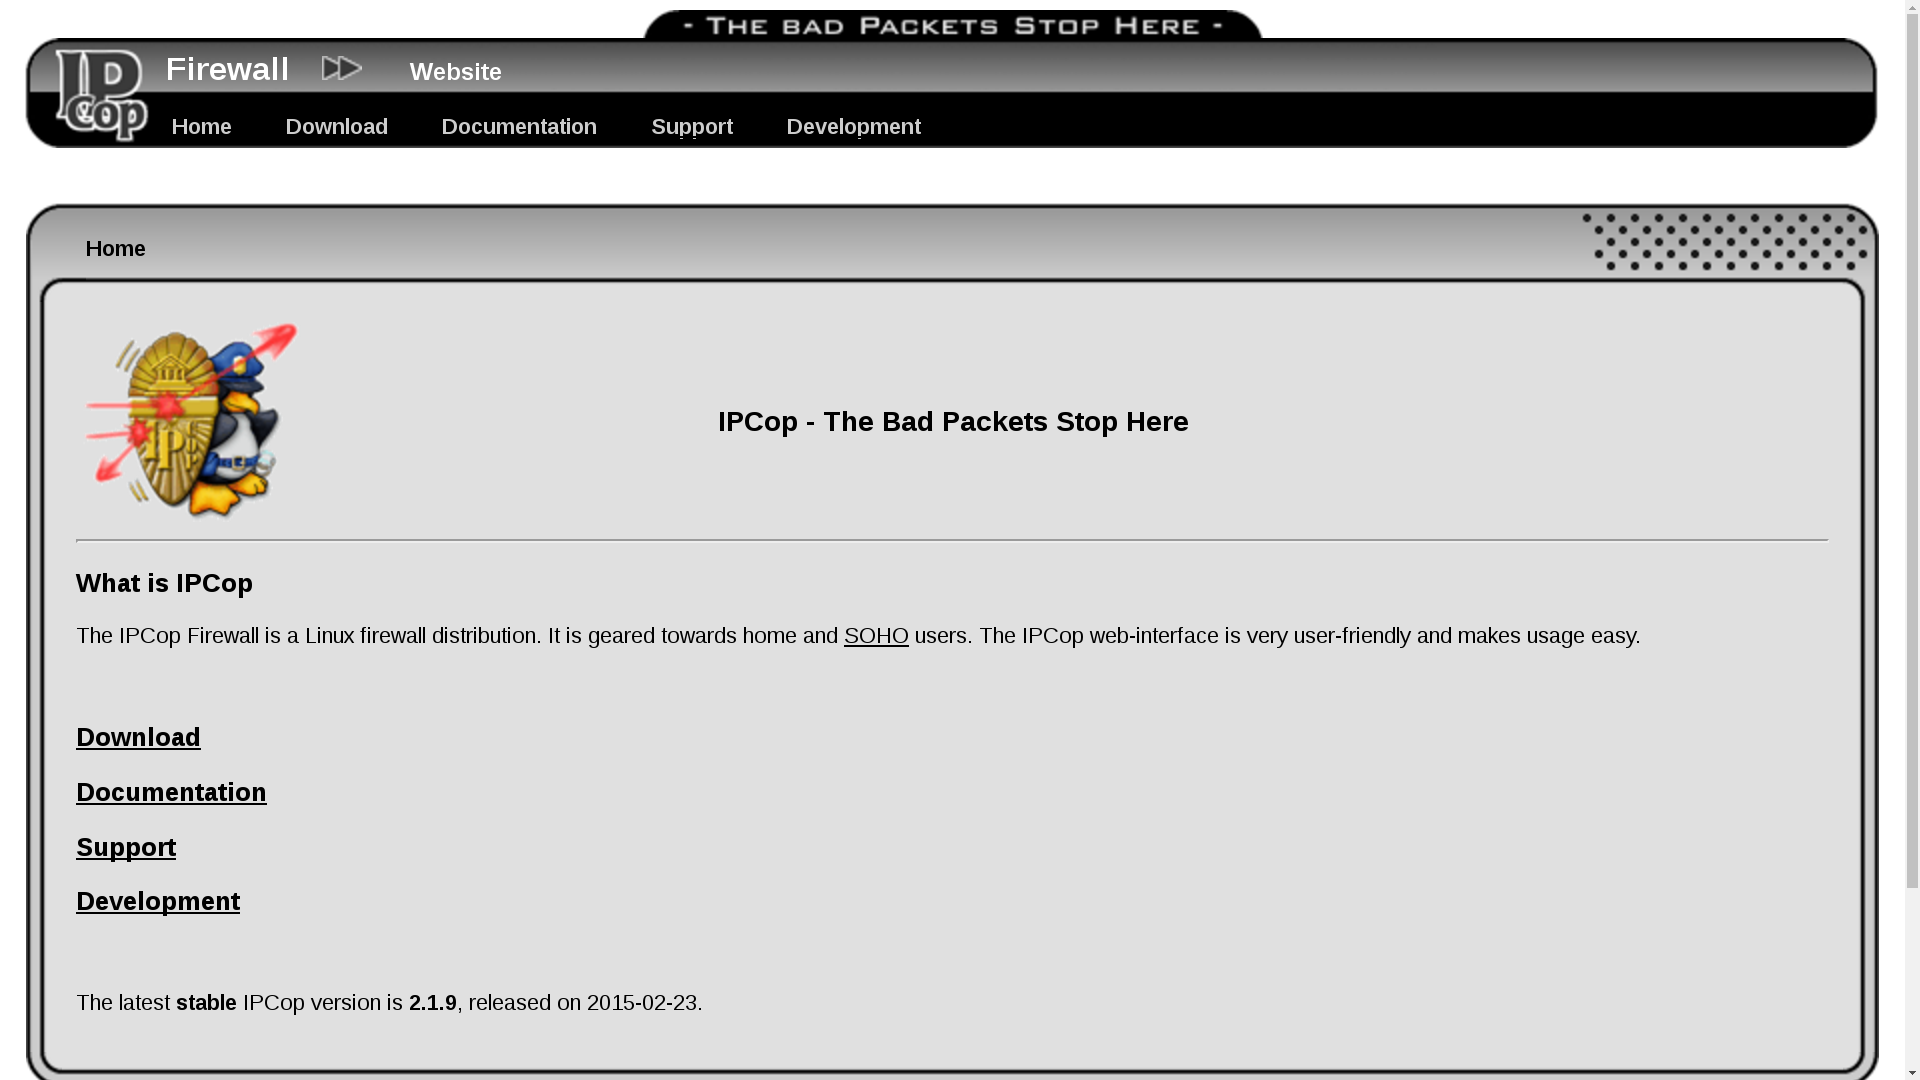
\includegraphics[keepaspectratio=true,height=1.10\textheight,width=1.00\textwidth,angle=0]{www-ipcop.png}

 \href{http://www.ipcop.org/}{IPCop} --- ``The IPCop Firewall is a Linux firewall distribution. It is geared towards home and SOHO users. The IPCop web-interface is very user-friendly and makes usage easy.''

\begin{itemize}
 \item Last release was 2015-02-23, well over a year ago.
 \item The i486 image doesn't boot all the way, gives video artifacts.
 \item All looks pretty old and crufty at this point.
\end{itemize}


\section{IPFire}
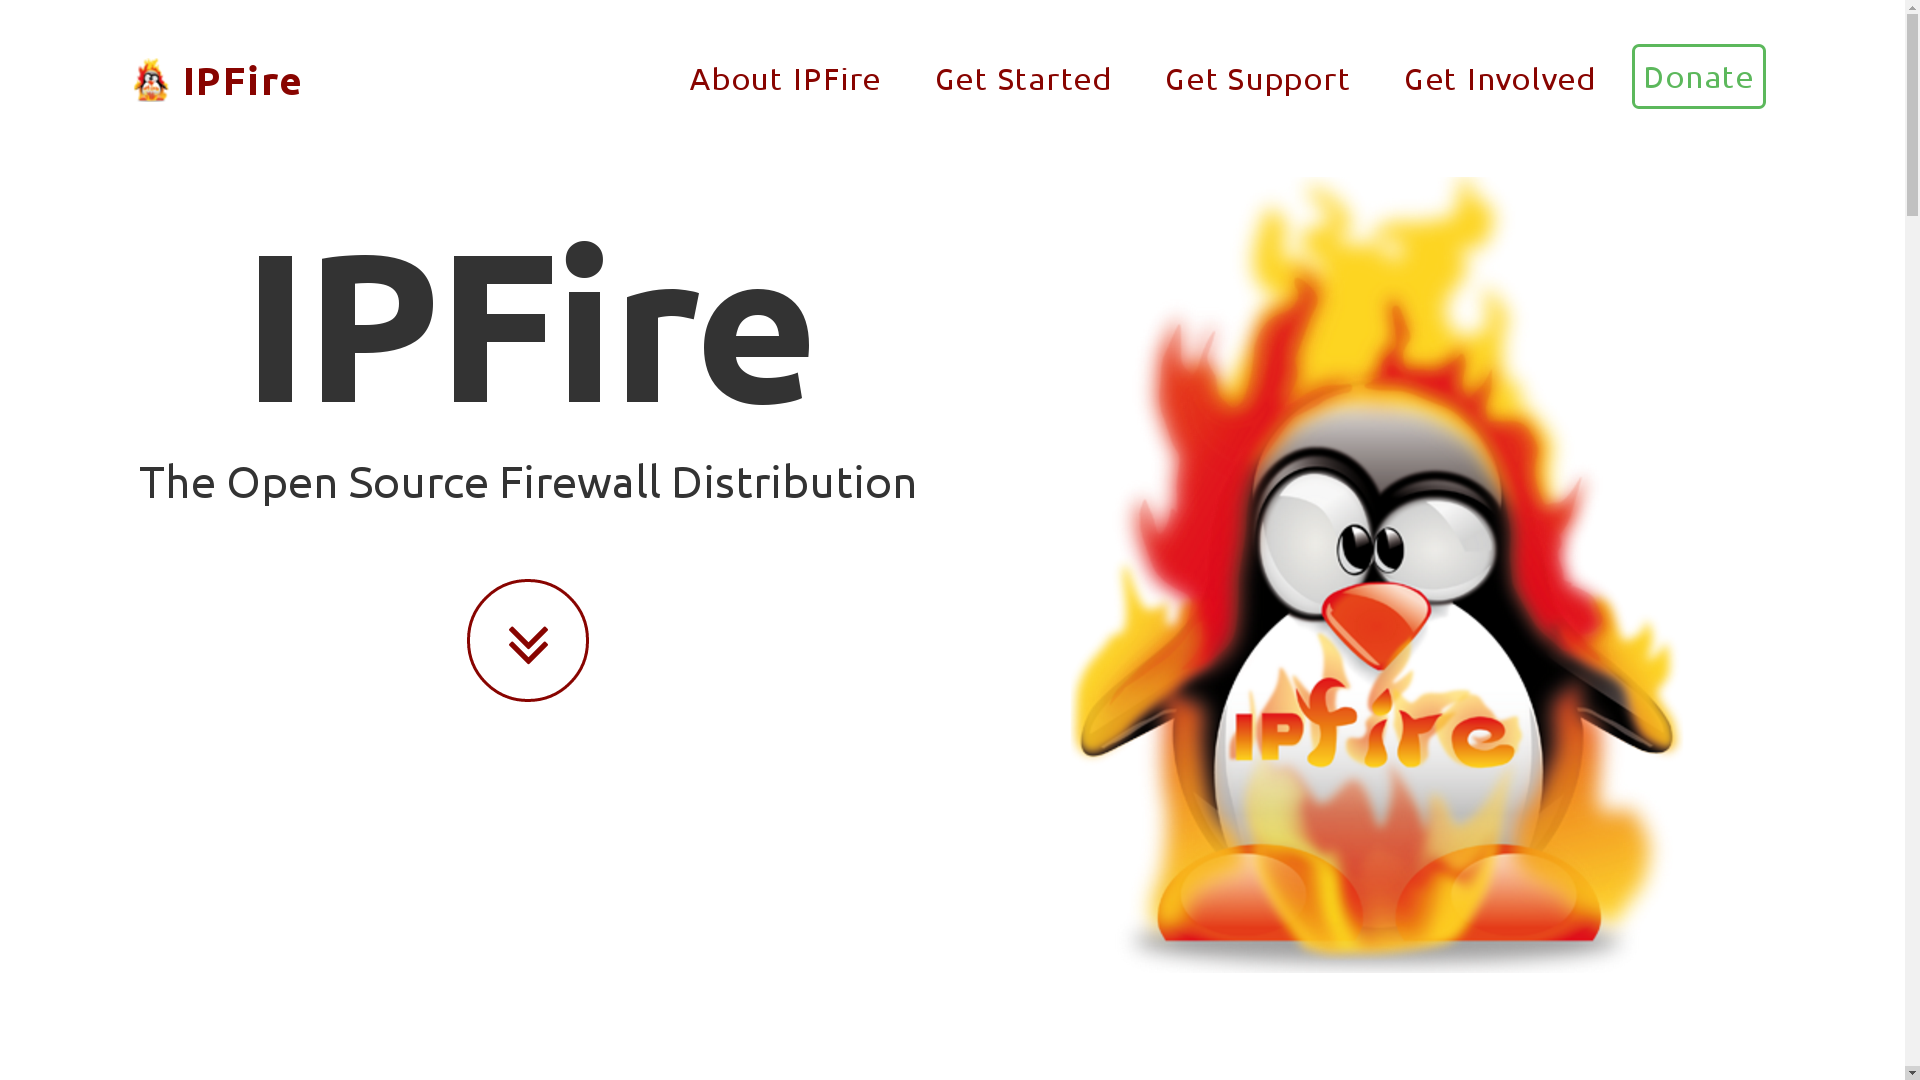
\includegraphics[keepaspectratio=true,height=1.10\textheight,width=1.00\textwidth,angle=0]{www-ipfire.png}

 \href{http://www.ipfire.org/}{IPFire} --- ``the professional and hardened Linux firewall distribution that is secure, easy to operate and coming with great functionality so that it is ready for enterprises, authorities, and anybody else.''

\begin{itemize}
 \item \url{http://downloads.ipfire.org/releases/ipfire-2.x/2.19-core103/ipfire-2.19.x86_64-full-core103.iso}
\end{itemize}


\section{OPNsense}
 \href{https://opnsense.org/}{OPNsense} --- ``the Open Source Firewall that is easy-to-use and protects your network``


\section{pfSense}
 \href{https://www.pfsense.org/}{pfSense} --- ``free, open source customized distribution of FreeBSD specifically tailored for use as a firewall and router that is entirely managed via web interface.''

